%  LaTeX support: latex@mdpi.com 
%  In case you need support, please attach all files that are necessary for compiling as well as the log file, and specify the details of your LaTeX setup (which operating system and LaTeX version / tools you are using).

%=================================================================
\documentclass[hydrology,article,submit,moreauthors,pdftex]{Definitions/mdpi} 

% If you would like to post an early version of this manuscript as a preprint, you may use preprint as the journal and change 'submit' to 'accept'. The document class line would be, e.g., \documentclass[preprints,article,accept,moreauthors,pdftex]{mdpi}. This is especially recommended for submission to arXiv, where line numbers should be removed before posting. For preprints.org, the editorial staff will make this change immediately prior to posting.

%--------------------
% Class Options:
%--------------------
%----------
% journal
%----------
% Choose between the following MDPI journals:
% acoustics, actuators, addictions, admsci, aerospace, agriculture, agriengineering, agronomy, algorithms, animals, antibiotics, antibodies, antioxidants, applsci, arts, asc, asi, atmosphere, atoms, axioms, batteries, bdcc, behavsci , beverages, bioengineering, biology, biomedicines, biomimetics, biomolecules, biosensors, brainsci , buildings, cancers, carbon , catalysts, cells, ceramics, challenges, chemengineering, chemistry, chemosensors, children, cleantechnol, climate, clockssleep, cmd, coatings, colloids, computation, computers, condensedmatter, cosmetics, cryptography, crystals, dairy, data, dentistry, designs , diagnostics, diseases, diversity, drones, econometrics, economies, education, electrochem, electronics, energies, entropy, environments, epigenomes, est, fermentation, fibers, fire, fishes, fluids, foods, forecasting, forests, fractalfract, futureinternet, futurephys, galaxies, games, gastrointestdisord, gels, genealogy, genes, geohazards, geosciences, geriatrics, hazardousmatters, healthcare, heritage, highthroughput, horticulturae, humanities, hydrology, ijerph, ijfs, ijgi, ijms, ijns, ijtpp, informatics, information, infrastructures, inorganics, insects, instruments, inventions, iot, j, jcdd, jcm, jcp, jcs, jdb, jfb, jfmk, jimaging, jintelligence, jlpea, jmmp, jmse, jnt, jof, joitmc, jpm, jrfm, jsan, land, languages, laws, life, literature, logistics, lubricants, machines, magnetochemistry, make, marinedrugs, materials, mathematics, mca, medicina, medicines, medsci, membranes, metabolites, metals, microarrays, micromachines, microorganisms, minerals, modelling, molbank, molecules, mps, mti, nanomaterials, ncrna, neuroglia, nitrogen, notspecified, nutrients, ohbm, particles, pathogens, pharmaceuticals, pharmaceutics, pharmacy, philosophies, photonics, physics, plants, plasma, polymers, polysaccharides, preprints , proceedings, processes, proteomes, psych, publications, quantumrep, quaternary, qubs, reactions, recycling, religions, remotesensing, reports, resources, risks, robotics, safety, sci, scipharm, sensors, separations, sexes, signals, sinusitis, smartcities, sna, societies, socsci, soilsystems, sports, standards, stats, surfaces, surgeries, sustainability, symmetry, systems, technologies, test, toxics, toxins, tropicalmed, universe, urbansci, vaccines, vehicles, vetsci, vibration, viruses, vision, water, wem, wevj

%---------
% article
%---------
% The default type of manuscript is "article", but can be replaced by: 
% abstract, addendum, article, benchmark, book, bookreview, briefreport, casereport, changes, comment, commentary, communication, conceptpaper, conferenceproceedings, correction, conferencereport, expressionofconcern, extendedabstract, meetingreport, creative, datadescriptor, discussion, editorial, essay, erratum, hypothesis, interestingimages, letter, meetingreport, newbookreceived, obituary, opinion, projectreport, reply, retraction, review, perspective, protocol, shortnote, supfile, technicalnote, viewpoint
% supfile = supplementary materials

%----------
% submit
%----------
% The class option "submit" will be changed to "accept" by the Editorial Office when the paper is accepted. This will only make changes to the frontpage (e.g., the logo of the journal will get visible), the headings, and the copyright information. Also, line numbering will be removed. Journal info and pagination for accepted papers will also be assigned by the Editorial Office.

%------------------
% moreauthors
%------------------
% If there is only one author the class option oneauthor should be used. Otherwise use the class option moreauthors.

%---------
% pdftex
%---------
% The option pdftex is for use with pdfLaTeX. If eps figures are used, remove the option pdftex and use LaTeX and dvi2pdf.

%=================================================================
\firstpage{1} 
\makeatletter 
\setcounter{page}{\@firstpage} 
\makeatother
\pubvolume{xx}
\issuenum{1}
\articlenumber{5}
\pubyear{2019}
\copyrightyear{2019}
%\externaleditor{Academic Editor: name}
\history{Received: date; Accepted: date; Published: date}
%\updates{yes} % If there is an update available, un-comment this line


\usepackage{threeparttable}
\usepackage{pgfplots}
\usepackage{natbib}
\PassOptionsToPackage{dvipsnames,svgnames,table}{xcolor}
\usepackage{xcolor,colortbl}
%tablenote:

%% MDPI internal command: uncomment if new journal that already uses continuous page numbers 
%\continuouspages{yes}

%------------------------------------------------------------------
% The following line should be uncommented if the LaTeX file is uploaded to arXiv.org
%\pdfoutput=1

%=================================================================
% Add packages and commands here. The following packages are loaded in our class file: fontenc, calc, indentfirst, fancyhdr, graphicx, lastpage, ifthen, lineno, float, amsmath, setspace, enumitem, mathpazo, booktabs, titlesec, etoolbox, amsthm, hyphenat, natbib, hyperref, footmisc, geometry, caption, url, mdframed, tabto, soul, multirow, microtype, tikz

%=================================================================
%% Please use the following mathematics environments: Theorem, Lemma, Corollary, Proposition, Characterization, Property, Problem, Example, ExamplesandDefinitions, Hypothesis, Remark, Definition
%% For proofs, please use the proof environment (the amsthm package is loaded by the MDPI class).

%=================================================================
% Full title of the paper (Capitalized)
\Title{A review of snow data assimilation  applied to mountain hydrology}
%\Title{A review on data assimilation of snow products applied to mountain hydrology}
% Author Orchid ID: enter ID or remove command
\newcommand{\orcidauthorA}{0000-0003-2395-2883} 

%\newcommand{\orcidauthorB}{0000-0000-000-000X} % Add \orcidB{} behind the author's name

% Authors, for the paper (add full first names)
\Author{Chloé Largeron $^{1,2}$\orcidA{}, Samuel Morin $^{1}$, Marie Dumont $^{1}$ and Aaron Boone $^{2}$}

% Authors, for metadata in PDF
\AuthorNames{Chloé Largeron, Samuel Morin, Marie Dumont, Aaron Boone}

% Affiliations / Addresses (Add [1] after \address if there is only one affiliation.)
\address{%
$^{1}$ \quad Univ. Grenoble Alpes, Université de Toulouse, Météo-France, CNRS, CNRM, Centre d'Études de la Neige, Grenoble, France\
$^{2}$ \quad CNRM, Université de Toulouse, Météo-France, CNRS, Toulouse, France
}

% Contact information of the corresponding author
\corres{Correspondence: chloe.largeron@meteo.fr}

% Current address and/or shared authorship
%\firstnote{Current address: Affiliation 3} 
%\secondnote{These authors contributed equally to this work.}
% The commands \thirdnote{} till \eighthnote{} are available for further notes

%\simplesumm{} % Simple summary

%\conference{} % An extended version of a conference paper

% Abstract (Do not insert blank lines, i.e. MAX 200 words\\) 
%CL: Abstract réduit pour ne pas excéder les 200 mots
\abstract{ Snow on the ground is a key component for land surface hydrology, especially in mountain areas where it governs the amount and timing of water availability in downstream areas. Snow is involved in climate feedbacks and contributes to natural hazards such as avalanches, so that monitoring and prediction of snow properties is required. The estimation of snow water equivalent (SWE) is crucial for hydrological applications, although it cannot be directly measured by satellites. This article describes \textit{in situ} and remote sensing options for measuring snow on the ground and highlights the associated limits and uncertainties of each observational technique.  %In contrast, SWE is a standard output of snowpack models driven by observed or forecast meteorological data. A large number of models represent snow processes with different degrees of complexity. Depending on the application, the physical processes of snow have to be represented in models leading to the development of more complex models such as detailed explicit process-based snow models. A description of snow evolution models with their related uncertainties are given. 
This article reviews current state-of-the-art methodologies used to optimally combined satellite measurements with snow models, through data assimilation. The choice of the method of snow data assimilation depends on the type of observations and the complexity of snow model used. The ability to determine snow water equivalent estimations also depends on the particular study region, and mountain areas are more challenging due to their complex topography. This article describes such issues and challenges, providing recommendations for future monitoring and prediction systems targeting snow in mountain regions for hydrological applications.}

%\abstract{A single paragraph of about 200 words maximum. For research articles, abstracts should give a pertinent overview of the work. We strongly encourage authors to use the following style of structured abstracts, but without headings: (1) Background: Place the question addressed in a broad context and highlight the purpose of the study; (2) Methods: Describe briefly the main methods or treatments applied; (3) Results: Summarize the article's main findings; and (4) Conclusion: Indicate the main conclusions or interpretations. The abstract should be an objective representation of the article, it must not contain results which are not presented and substantiated in the main text and should not exaggerate the main conclusions.}

% Keywords
%CL: A compléter au fur et à mesure
\keyword{Data assimilation; Snow water equivalent; Remote sensing, Snow models}

% The fields PACS, MSC, and JEL may be left empty or commented out if not applicable
%\PACS{J0101}
%\MSC{}
%\JEL{}

%%%%%%%%%%%%%%%%%%%%%%%%%%%%%%%%%%%%%%%%%%
% Only for the journal Diversity
%\LSID{\url{http://}}

%%%%%%%%%%%%%%%%%%%%%%%%%%%%%%%%%%%%%%%%%%
% Only for the journal Applied Sciences:
%\featuredapplication{Authors are encouraged to provide a concise description of the specific application or a potential application of the work. This section is not mandatory.}
%%%%%%%%%%%%%%%%%%%%%%%%%%%%%%%%%%%%%%%%%%

%%%%%%%%%%%%%%%%%%%%%%%%%%%%%%%%%%%%%%%%%%
% Only for the journal Data:
%\dataset{DOI number or link to the deposited data set in cases where the data set is published or set to be published separately. If the data set is submitted and will be published as a supplement to this paper in the journal Data, this field will be filled by the editors of the journal. In this case, please make sure to submit the data set as a supplement when entering your manuscript into our manuscript editorial system.}

%\datasetlicense{license under which the data set is made available (CC0, CC-BY, CC-BY-SA, CC-BY-NC, etc.)}

%%%%%%%%%%%%%%%%%%%%%%%%%%%%%%%%%%%%%%%%%%
% Only for the journal Toxins
%\keycontribution{The breakthroughs or highlights of the manuscript. Authors can write one or two sentences to describe the most important part of the paper.}

%\setcounter{secnumdepth}{4}
%%%%%%%%%%%%%%%%%%%%%%%%%%%%%%%%%%%%%%%%%%
\begin{document}
%%%%%%%%%%%%%%%%%%%%%%%%%%%%%%%%%%%%%%%%%%

%For any questions, please contact the editorial office of the journal or support@mdpi.com. For LaTeX related questions please contact latex@mdpi.com.
%The order of the section titles is: Introduction, Materials and Methods, Results, Discussion, Conclusions for these journals: aerospace,algorithms,antibodies,antioxidants,atmosphere,axioms,biomedicines,carbon,crystals,designs,diagnostics,environments,fermentation,fluids,forests,fractalfract,informatics,information,inventions,jfmk,jrfm,lubricants,neonatalscreening,neuroglia,particles,pharmaceutics,polymers,processes,technologies,viruses,vision


\section{Introduction}

Snow on the ground is an important component of the climate system, which drastically modifies the exchange of mass, momentum and energy between the soil and atmosphere \citep{Groisman_1994,Qu_2006,Flanner_2011}. It plays a particular role in the Earth system through its physical and optical properties. The surface energy and moisture balance is also influenced by freeze/thaw cycle and their representation in model are essential for modelling the thermal characteristics and the hydrological cycle \citep{Gouttevin_2012}. The low thermal conductivity of snow makes it a particularly insulating Earth surface medium, with major implications for underlying ground temperature. The presence of snow on the ground also changes the surface albedo and the aerodynamic roughness \citep{Hansen_2004,Flanner_2006,Qu_2014,Hall_2006}. 

%Hydrology
At regional and local scale, snow on the ground  plays a major role in the hydrological cycle. Seasonal snow cover is the primary water source for human use and ecosystems in mountains regions, where the runoff is heavily dependent on snowmelt amount and timing \citep{Bales_2006,Bowling_2003}. Monitoring and predicting the mass of the snow cover, most often referred to as the snow water equivalent (SWE), is particularly important for water resources management with major implications for natural hazards (avalanches, snowmelt floods) \citep{Sui_2001,Finger_2012,Viviroli_2011,Freudiger_2014}.
% A good estimation of SWE measurement is an essential requirement to properly forecast the river-flow during the snowmelt period. 

%in situ
\textit{In situ} observations are essential to monitor the evolution of the snowpack (snow depth, SWE, vertical profile of density and temperature) and their surface properties (albedo, surface temperature) \citep{Morin_2012,Lejeune_2018}. \textit{In situ} snow datasets are vital for the evaluation of snow model processes and satellite products \citep{Brun_1992,Vionnet_2012,Krinner_2018}. Point measurements are inherently limited in total number and spatial extent and do not allow to provide information on the spatial heterogeneity.%, thus making the use of satellite observations an indispensable tool. \textit{In situ} snow datasets are vital for the evaluation of snow model processes and satellite products.
%The latter is crucial to forecast hydrological and avalanches risks, although it cannot be directly measured by satellites. 


%Importance données satellite
%Voir intro papier COST
Satellite observations are crucial for monitoring the evolution of the snow cover over large areas \cite{DeLannoy_2012}. Satellite sensors address different measurement wavelength and employ various operating principles (active or passive). Multi-spectral images by optical sensors focus on the visible and near infra-red domain with a spatial resolution ranging from 50 cm to 500 m. Under cloud-free conditions, these images provide snow cover extent information, but also information on albedo and impurities as well as snow grain size \cite{Hall_1995,Hall_2007,Dietz_2012,Gascoin_2015}. Observations of snow cover areas that are particularly valuable in mountain regions have shown an improved performance of hydrological models \cite{Lee_2005,Immerzeel_2009,Finger_2015}.

Conventional passive microwave measurements have the ability to detect through clouds and during the night. However, the  spatial resolution of around 25 km is too coarse to allow suitable measurements of snow distribution in complex snow terrain, such as mountainous regions \cite{Foster_2005,Cordisco_2006,Tedesco_2010,Li_2014}. Active microwave satellites (radar) emit a microwave signal and then measure the backscattered energy. Their high spatial resolution (spanning from a few meters to a few tens of meters) is attractive for monitoring snow in complex terrain, but the radar signal contains information that is only indirectly related to the snow conditions, and affected by other land surface elements (vegetation, topography etc.) \cite{DeLannoy_2012,Conde_2019}.



%Representation dans les modèles
The representation of snow on the ground in land surface models is crucial in view of its role in the climate system and the hydrological cycle. Snow was first included into land surface models (LSMs) to obtain improved time varying estimations of the surface energy balance over cold regions \cite{Loth_1993,Lynch_1994,Douville_1995,Yang_1998,Slater_1998}. In order to better represent and account for the interactions between snow and the climate system, more complex representations of the physical properties of the snow have been progressively incorporated into LSMs \citep{Brun_1992,Lehning_1999,Boone_2001}. %,Vionnet_2012,Wang_2013}. 
Depending on the application, models include different levels of complexity of the snowpack, from single layer models to multi-layer schemes including micro-structure such as Crocus \citep{Vionnet_2012}.

%combiner obs et modèles
Observations and numerical simulations represent two sources of information that can be exploited simultaneously. Data assimilation proceeds through the optimal combination of observed and simulated snow properties. This technique can be used to improve initial conditions of the snowpack for operational numerical weather or hydrological prediction. It can also be used for the estimation of optimal model parameters. In data assimilation, observations are used to correct the physical state given by a model in order to improve the overall representation of a particular system \cite{Andreadis_2006,Clark_2006,Leisenring_2011,Nagler_2008,Liu_2013}.
Various data assimilation methods exist which are each characterised by certain advantages and difficulties. Choosing the appropriate method depends on the type of model and observation used, and on the target application of modelling system.

This paper aims to provide optimal data assimilation methods for snow hydrology applications in mountainous regions, based on the data assimilation methods, snow models and satellites limitations. This paper describes (1) the different types of snow observations and their uncertainties spanning from in-situ methods to optical and microwave satellites, (2) the different complexity of snow evolution models, where the choice of the complexity of a model depends on the required applications, and  (3) different data assimilation methodologies, including a description of the limits of each method for snow applications. %, where a state of the art is given by application. 


\section{Observations}

\textit{In situ} measurements and satellites observations supply large observations tools to monitor the snowpack. \textit{In situ} snow measurements provide critical data for characterizing the snow cover. However, the scarcity and representativity issues of point-scale \textit{in situ} data makes the use of satellite observation unavoidable to monitor snow spatial variability. The choice of a given observation type depends on the required information and the purpose of the study.

This section describes the different methods of observations commonly used to determine the evolution of the snow cover, emphasising on snow water equivalent because of its critical relevance to mountain snow hydrology. Advantages and inconvenients will be described for each type of observation. 

\subsection{\textit{In situ} observations}

%Parler des mesures automatiques manuelles. Donner techniques du SWE.
Site measurements describe the characteristics of the snow cover at a given locationat only one point (fixed instruments) or over a defined area such as terrestrial laser scanning (\textit{i.e} camera, terrestrial laserscan). \textit{In situ} measurements are performed automatically by fixed measuring instruments which provide continuous data or discontinuous data when it requires manual intervention. \textit{In situ} observations are performed either at conventional, operational meteorological stations and at experimental snow sites, which are dedicated to monitor the evolution of the snowpack.%, which is crucial to the understanding of the evolution of the snow cover.

\subsubsection{Meteorological stations}
Weather stations provide continuous meteorological information on a site such as wind speed, temperature, incoming radiation, specific humidity and precipitation rate. Severals stations as WMO synoptic stations can also provides snow measurements such as snow cover fraction (visually estimated), snow height (measured), snow density (measured with a snow tube) and snow depth (manual or sonic sensors).  The weather stations cover the whole globe with a wide degree of heterogeneity. The studies of \citet{Ripper_2015snowpex} highlight a high density of weather stations in Europe and North America while Russian weather stations are more scarce.  


\subsubsection{Experimental snow sites}

The monitoring of the snowpack in conventional weather stations is often insufficient for improved process understanding. To overcome this lack of informations, experimental snow sites have been installed and include instruments specific for snow measurements. These sites contain automatic instruments providing daily and hourly measurements of meteorological meteorological and snow variables such as presence of snow, snow depth, SWE, snow density albedo and runoff \citep{Pirazzini_2018}. Discontinuous measurements are often performed seasonally, especially during winter, \textit{e.g.} snow stratigraphy profile \citep{Morin_2012}. The structure of snow grain size is also determined following the International Classification for Seasonal Snow on the Ground (ICSSG)  \citep{Fierz_2009}. Measurements from snow sites such as Sodankylä (Finland), Weissfluhjoch (Switzerland), Caribou Creek (Canada), CARE
(Canada), Formigal (Spain), Forni
Glacier (Italy), Col de Porte (France), Gochang (Korea) and Pyramid Observatory (Nepal/Italy) have been analysed during the WMO Solid Precipitation Intercomparison Experiment (SPICE) \citep{Smith_2017}. Only few experimental study sites of snow containing all the meteorological and snow variables required to determine the surface energy balance in the presence of snow exist. These sites, such as the experimental Col de Porte site are particularly relevant to study the evolution of the snow \citep{Morin_2012,Lejeune_2018}. %Only severals experimental study sites of snow exists, such as study site of snow is the Col de Porte (CDP) experimental site, located in the French Alps in the Chartreuse mountain range (Fig \ref{CdP}, 1325 m alt.). This site is particularly relevant to study the evolution of the snow \citep{Morin_2012,Lejeune_2018}. Experimental snow sites contain all the meteorological and snow variables required to determine the surface energy balance in the presence of snow. 
It has often been used for snow model evaluation \citep{Brun_1992,Vionnet_2012,Decharme_2016,Wang_2013,Krinner_2018}. 
Other experimental sites can be used for specific purpose as the largely exposed to strong wind experimental site of the Col du Lac Blanc (2720 m alt.) in the French Alps, which is perfectly suitable to study and measure blowing snow events \citep{Vionnet_2013,Guyomarch_2018}. 


%COST snow obs DA: \cite{Helmert_2018} 

\subsubsection{Methods of SWE measurements}
Various methods can be used to measure SWE, automatically and manually. SWE manual measurements are based on bulk density samples made with a snow sampling tube (more detailed description is given in the study of \citet{Leppanen_2016}). The lack of available manual measures has conducted to use more often automatic measurements.
The most used technique for continuous SWE measurements is the snow pillow \citep{Serreze_1999,Smith_2017}, where the pressure sensors measure the hydrostatic pressure of the snow \citep{Beaumont_1965}. However, this method has large uncertainties, especially when the snowpack contains liquid water. Gamma-ray sensor can also be used to measure SWE continuously. Gamma-ray sensors originally used a radiation source \citep{Harding_1986}. For safety and environmental reasons, this instrument has been gradually replaced by natural emitted radiation such as passive gamma radiation (Potassium and Thallium) sensors and cosmic-ray nivometers (NRC). This latter uses the harmless natural cosmic-ray to directly estimate SWE \citep{Choquette_2008,Martin_2008}. An assessement of the different SWE measurements is detailed during the WMO SPICE experiment \citep{Smith_2017}. The uncertainties of each method are described in the following section.

%\begin{figure}
%	\centering
%	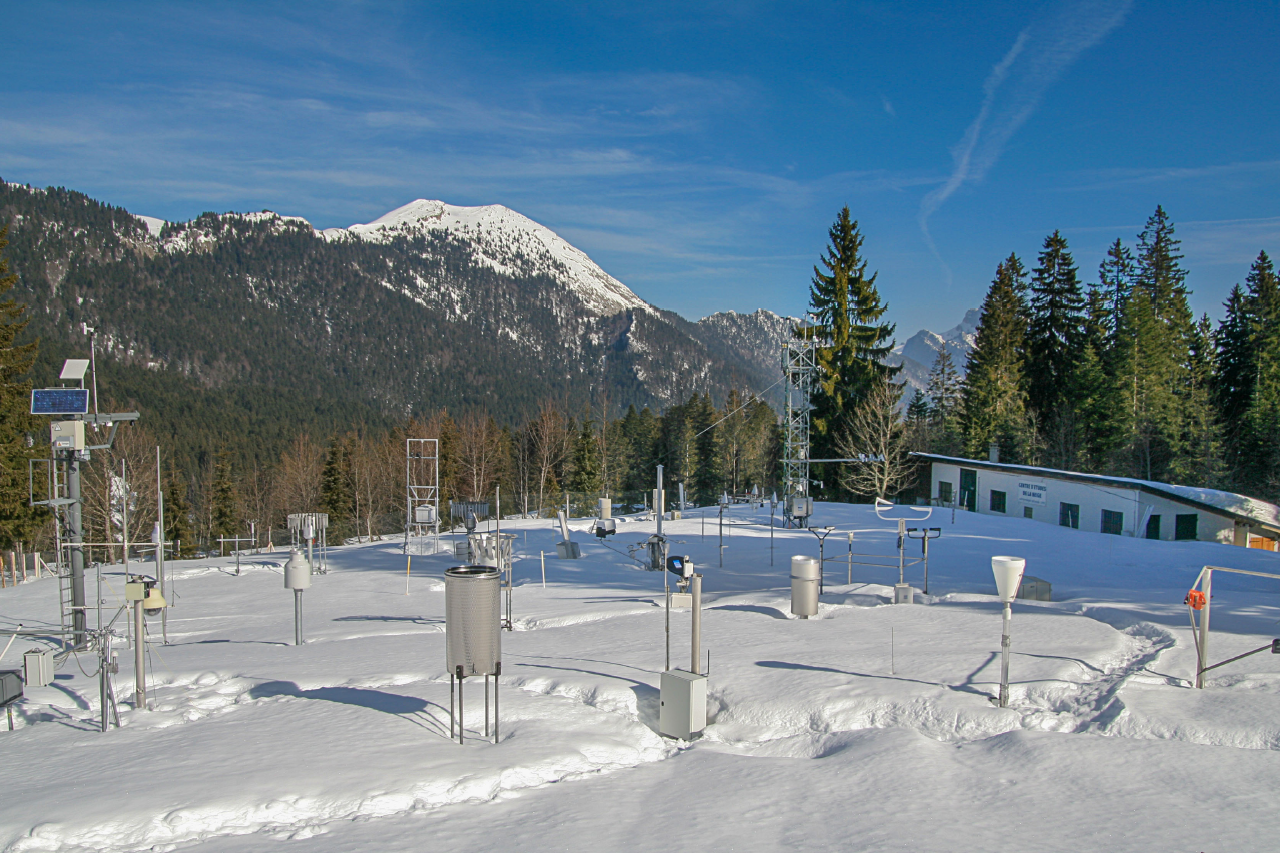
\includegraphics[scale=0.2]{Figures/CdP}
%	\caption{Picture of the Col de Porte site located in the Chartreuse mountain range, French Alps.}\label{CdP}
%\end{figure}


\subsubsection{Measurements uncertainties}
%parler des incertitudes sur les différentes méthodes de mesures du SWE.

The uncertainties of \textit{in situ} datasets is not only due to the intrinsic uncertainty of snow measurements. In mountain environments, the large variability of snow height around a given observation point requires that this point scale data is used with great caution \citep{Grunewald_2013}. 
In the studies of \citet{Lafaysse_2017} on snow depth measurements, the instrumental error is low (about 1 cm) compared to the spatial variability of snow depth of the surrounding environment (up to 20 cm). The uncertainty of SWE measurements can be of the same order of magnitude than their spatial variability \citep{Smith_2017,Lafaysse_2017}. 

Measurements uncertainties of SWE varies also with the choice of instrumentation used. The uncertainty of snow tube compared to a layer integrated snow pit measurement have been estimated to an average underestimation of 7.1 $\%$ \citep{Sturm_2010}. The largely used snow pillow SWE measurements, suitable especially in cold climate as Canada, contains uncertainties range from 6-12 $\%$ in optimal conditions. The uncertainty of snow pillow measurements increases in the presence of liquid water in the snowpack leading to be particularly unsuitable during the snowmelt season \citep{Smith_2017,Engeset_2000}. The lowest uncertainty of SWE measurement is obtained by cosmic-ray nivometers (NRC), where the accuracy is around 5-10 $\%$ \citep{Lafaysse_2017, Smith_2017}. This methods has shown a r$^{2}$ values higher than 0.90 compared to manual measurements for Finland and Canadian sites \citep{Smith_2017}, where the automated and manual sensors have been made with a distance varying from 5 to 25 m. The difference observed between the measurements can partly be explained by the spatial variability. The SWE sample uncertainties estimated between 5-10 $\%$ has also to be taken into account. 

%SWE is the most important unsolved problem in snow hydrology especially in mountain regions \citep{Dozier_2016}. The combination of the use of \textit{in situ} datasets and remote sensed data (satellite or terrestrial) is crucial for large scale studies.
%complementarity satellite and in situ

%%%%%%%%%%%%%%%%%%%%%%%%%%%%%%%%%%%%%%%%
%%%%           Satellites           %%%%

\subsection{Satellite remote sensing observations}

Combined with \textit{in situ} datasets, remote sensing observations are crucial for monitoring the snow cover evolution over large areas. A wide variety of satellite sensors exists with various spatial resolutions composed by different category of wavelengths. The choice of remote sensing techniques for snow products varies with the desired temporal and spatial resolution. This section describes the different types of satellite sensors (optical and microwave satellite sensors) used for monitoring snow hydrology and indirectly SWE observations. Examples of space-borne used in related snow studies with their general properties classified by type of satellites sensors are summarised in Table \ref{tab:satellites}.


\subsubsection{Optical satellites} %SCA/SCF/SE et indirectement SWE et delta h
%subsubsection{Snow cover extent}

\paragraph{Monoscopic optical satellites}
Optical sensors use a multi-spectral imaging system in the visible and infrared domain covering a large spectral resolution. By design, data is only available during daytime and under cloud free conditions. The spatial resolution of optical satellites varies from 50 cm to 1 km.%Since snow has a high reflectance in the visible spectrum and in the short wave infrared, these satellite measurements are useful to provide observations of the surface area covered by snow. 
Optical satellites are largely used to monitor the Snow Cover Area (SCA) given a binary information on the presence or absence of snow in a given pixel, and the Snow Cover Fraction (SCF), which provides the percentage coverage of snow in a given pixel. This latter calculation is often based on spectral unmixing methods, where the total reflectance in a pixel correspond to the sum of the reflectance due to snow, rock and vegetation. %Another method to produce SCA map has been used by \cite{Hall_1995}. 
\citet{Hall_1995} have computed SCF based on the Normalized Difference Snow Index (NDSI) (Eq. \ref{ndsi}), which uses reflectance data from both visible (vis, green band) and short wave infrared (swir) \citep{Sirguey_2009}. Snow mapping by optical satellites in mountainous region is affected by errors induced by the complex terrain. The high reflectance of snow varies widely depending on the wavelength and the structure of the snow. It can be easily identified with visible bands satellites in comparison with snow-free areas. It can detect snow impurities and snow grain size in the visible and infrared range but cannot detect liquid water and then direct SWE estimations is not possible without assimilation of snow products \citep{Mary_2013}. Optical satellites are also used to retrieved daily snow albedo, e.g. based on MODIS products \citep{Klein_2002}. The exploitation of these images results difficult to interpret in forest and shadows areas, \textit{i.e.} in mountain locations.
%An alternative to optical satellite data is the use of camera to monitor snow cover fraction in several areas \citep{hinkler2002, bernard2013}. 

 



\begin{equation}
NDSI=\dfrac{\rho_{vis}-\rho_{swir}}{\rho_{vis}+\rho_{swir}}
\label{ndsi}
\end{equation}

\paragraph{Stereoscopic optical satellites}

Stereoscopic satellites (Pleiades 1a, 1b and SPOT5) capture a specific region with different angles of view with a very high resolution (VHR, 50 cm-2 m). These images can be used for 3D mapping by photogrammetry, thereby providing topographic informations. However, these sensors cannot provide daily imagery. The acquisition images is on request only. The tri-stereoscopic Pleiades satellite has been used to retrieve snow depth over an open alpine catchment, by comparing winter and snow-free images \citep{Marti_2016}. However, the uncertainty of snow depth measurement is estimated to be on the order of 50 cm \citep{Marti_2016}. There remains a substantial uncertainty on the final snow volume at the watershed scale. The remote sensing Lidar technology (for in situ, unmanned aerial vehicles, plane or satellite - Ice Sat, Ice Sat 2, e.g. \citep{kwok2008, deems2013}) can also be used for high resolution snow depth mapping by difference between snow-free and snow-covered dates. The calculation of snow depth remains uncertain especially in steep slopes \citep{Deems_2006}.
%%% REFS ASO ??? DEMANDER A CESAR ???
%CL:  ASO?


The most used satellites to detect snow are classified in the Fig. \ref{sat} as a function of their revisit time vs. their spatial resolution.  High resolution satellites used for snow cover mapping (SPOT 6/7, Sentinel 2, Landsat 8, Pleiades 1A and 1B) are limited by the revisit time (Fig. \ref{sat}). For the case of SPOT 6/7 and Pleiades, the acquisition of satellites images are performed on demand, and can be superseded by higher priority requests. Optical satellite data with most frequent revisit times are currently MODIS, PROBA-V, Sentinel 3 and VIIRS. Higher revisit times increase the probability to obtain a cloud-free image. 
%From these satellites images, the finest spatial resolution is obtained by the MODIS data products. 
MODIS data are largely used to retrieve snow cover fraction and snow albedo covering the entire earth at a near daily frequency \citep{Klein_2002,Masson_2018}. 



\begin{figure}[h]
	\centering
	%	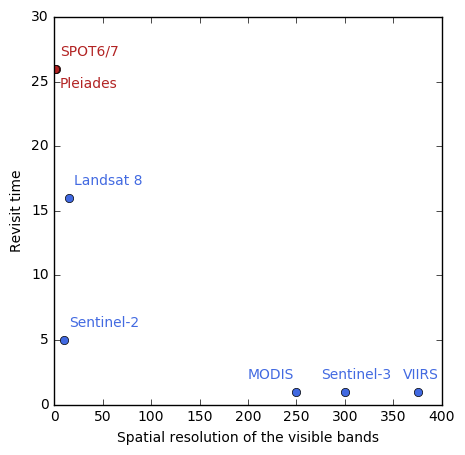
\includegraphics[scale=0.72]{Figures/sat}
	%Fig Optical satellites:

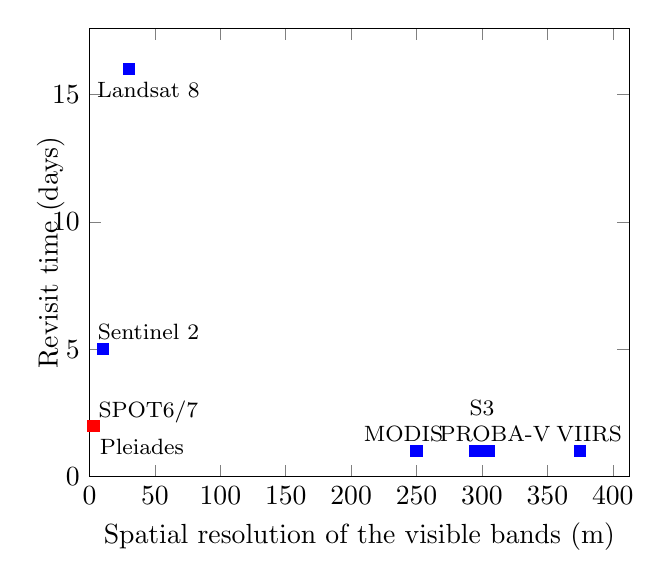
\begin{tikzpicture} 
	\begin{axis}[% 
		%coords={(xy): \thisrow{label}},%
		ylabel style={yshift=-0.4cm}, %shifting the y line text
	%	ylabel shift = 40 pt,
		ymin = 0,
		xmin=0, 
		xlabel={Spatial resolution of the visible bands (m)}, 
		ylabel={Revisit time (days)},
		xtick={0,50,100,150,200,250,300,350,400},
		ytick={0,5,10,15,20},
		scatter/classes={%
		b={mark=square*,blue},%
		r={mark=square*,red}}]
%	set(y, 'Units', 'Normalized', 'Position', [-2, 0.5, 2]);
		\addplot[scatter,only marks,%
		scatter src=explicit symbolic,
		point meta=explicit symbolic]%
		table[meta=label] {
    %    table[meta index=2]
			x y label 
			250 1 b  
			295 1 b
			305 1 b
			375 1 b
			3   2 r
			3   2 r
			30  16 b
			10  5 b
			};
	%	\node at (axis cs:0,0)

		\node [above] at (axis cs:  45,  14.5) {\footnotesize Landsat 8};
		\node [above] at (axis cs:  45,  1.7)  {\footnotesize SPOT6/7};
		\node [above] at (axis cs:  40,  0.5)  {\footnotesize Pleiades};
		\node [above] at (axis cs:  45,  5)    {\footnotesize Sentinel 2};
		\node [above] at (axis cs:  240,  1)   {\footnotesize MODIS};
		\node [above] at (axis cs:  300,  2)   {\footnotesize S3};
		\node [above] at (axis cs:  310,  1)   {\footnotesize PROBA-V};		
		\node [above] at (axis cs:  382,  1)   {\footnotesize VIIRS};
	\end{axis}
\end{tikzpicture}

%\begin{tikzpicture} 
%	\begin{axis}[% 
%	scatter/classes={% 
%		a={mark=square*,blue},% 
%		b={mark=square*,red},% 
%	}]
%%		xlabel={Spatial resolution of the visible bands (m)}, 
%%		ylabel={Revisit time (days)}]
%	\addplot[scatter,only marks,% 
%	scatter src=explicit symbolic]% 
%	table[meta=label] {
%	x y label
%	0.1 0.15 a 
%	0.85 0.52 b 
%	0.76 0.5 b 
%	0.55 0.32 c
%	}; 
%	\end{axis} 
%\end{tikzpicture}		
	\caption{Representation of optical satellites revisit time (days) vs. the corresponding spatial resolution of the visible bands (m).}\label{sat}
\end{figure}

% Stereoscopic optical satellites provide high spatial resolution images (1 m) with different angles of view allowing to get 3D images by photogrammetry. However, stereoscopic satellites cannot do daily records and have limited revisit time or available acquisitions images. The estimation of snow depth with optical satellite can be made by comparison between snow and snow-free period but with a high uncertainty \citep{Marti_2016}. These satellite can not directly measures SWE estimations.
%In summary, optical satellites are largely used to produce snow cover maps with a wide range of resolution and revisit time. Satellite sensors with the highest spatial resolution (1 m), such as Pleiades and SPOT 6/7, have a limited available images (25 days cycle). Conversely, the highest frequency satellites (daily), such as MODIS, have a coarser spatial resolution (250-500 m).





\subsubsection{Passive microwave}
%a citer Snow cci
%a citer : Foster_2005 uncertainty in passive microwave SWE obs:


Passive microwave sensors (10$^{-3}$ to 1 m wavelength) has the advantage to provide data under all atmospheric conditions, during daytime and nighttime.  The spectral luminance energy measured by passive microwave sensors allow to calculated brightness temperature which can be used to estimate snow depth \citep{Chang_1982}. The estimation of SWE is based on the brightness temperature alone or combined with snow depth and snow density measurements \citep{Chang_1987,Cho_2017,Davenport_2012}.

Passive microwave satellites have proven to be useful for monitoring snow cover at global and regional scales \citep{Armstrong_1995}. These satellites are used to observe the surface and can be used for surface melting observations \citep{Picard_2006}. Studies during the GLOBSNOW project have used a combination of passive microwave and meteorological stations to produce daily SWE map \citep{Luojus_2014}. These types of satellites can also detect surface melting and can easily be used to produce melting snow map. The characteristics of passive microwave satellites used in snow studies is summarised in the studies of \citet{Konig_2001}. The coarse spatial resolution of passive microwave sensors (around 25 km) does not allow to represent fine scale processes, restraining this method for complex mountainous areas. The passive microwave measurement of SWE are associated to uncertainties, which are mainly caused by the vegetation cover, the unaccounted impact of snow micro-structure (density, layering, snow grain size) and errors related to the brightness temperature calibration \citep{Foster_2005}. The more recent satellites (AMSR-E, AMSU-A, AMSU-B) present a finer spatial resolution and a larger swath width allowing a better coverage efficiency. Due to the high spatial variability of mountains regions, passive microwave sensors measurements are often inadequate. 


%These measurements are often used to estimate snow depth and snow water equivalent. %However, the measurement of SWE requires to know the conditions of the snowpack. 
%The errors associated to the passive microwave measurement of SWE are mainly caused by the vegetation cover, the unaccounted impact of snow microstructure (density, layering, snow grain size) and errors related to the brightness temperature calibration. \citet{Foster_2005} have shown, in north America, that the error of SWE estimate due to grain size range from 9-18 mm\,w.e. (kg\,m$^{-2}$), the vegetation-induced error is generally low (3 kg\,m$^{-2}$) except in the tundra (up to 18 kg\,m$^{-2}$) and the brightness temperature error range from 6-15 kg\,m$^{-2}$. The maximum errors approached 24 kg\,m$^{-2}$.


%In order to reduce the uncertainties, different methods exist to combine microwave measurement with \textit{in situ} and/or optical measurements (see section \ref{section_DA}). 

%In summary, passive microwave satellite has the advantage to provide data under all atmospheric conditions, during daytime and nighttime. However, the coarser resolution restrain this method for complex mountainous areas. The estimation of SWE is based on the brightness temperature alone or combined with snow density measurements. Studies use a combination of \textit{in situ}, optical and microwave measurements and model to reduce SWE estimations uncertainties. SWE products uncertainties are related to observations uncertainties, which are considered to be error-free in the direct insertion method (see section \ref{section_DA}) \citep{Fletcher_2012}. In this study, snow depth was underestimated by a factor of 5 for some stations although accumulation and melt is consistent. These types of satellites detect surface melting and can easily be used to produce melting snow map.


\subsubsection{Active microwave}%radar Sentinel1 ? bande Ka, Ku, C
%pouvoir de penetration dans le manteau neigeux determine structure des couches
% - Propr. radar utile pour la neige


% - Etudes qui utilise radar pour la neige : applications possibles et limitations


Active microwave radar (RAdio Detection And Ranging) contains their own source of radiation. The detection of the scattered signal emitted by the active radar provides information on surface structure such as roughness of snow. Like passive microwave, radars are not disturbed by cloud covers and can record during day and night. %The very high resolution imaging is obtained with the active imaging SAR allowing the exploitation of snowpack monitoring in mountainous regions. SAR is also a main tool for mapping and monitoring the extent of wet snow areas. The use of SAR data combined with algorithms allows snowmelt map production \citep{Shi_1994,Eckerstorfer_2016}. 
Radar allows to determine structure properties of snowpack layers.
It has been used for the retrieval of snow wetness, snow depth and then SWE estimations \citep{Schmid_2014}. The radar signal is sensitive to the presence of liquid water, leading to higher backscatter for wet snow conditions \citep{Magagi_2003}. 


The very high resolution imaging (up to 1m) is obtained with the active imaging Synthetic-aperture radar sensors (SAR) that are suitable for dry and wet snow and can be used to monitor the snowpack during snowmelt period. Several studies have used SAR imaging system for the production of snowmelt map  \citep{Shi_1994,Eckerstorfer_2016}. The backscatter signal of the SAR sensors allow to estimate the snow depth but the state of the snow such as the humidity of the snow must be known beforehand. The estimation of surface elevation is usually characterised by non-imaging microwave radar sensors altimeters and scatterometers. A comparison of the different characteristics of SAR sensors and passive microwave is given in the studies of \citet{Konig_2001}.
%Active microwaves satellites cannot estimates directly the SWE but its estimation is possible through the use of radiative transfer models \citep{Marshall_2005}.
The high spatial and temporal resolution of SAR sensors makes their use potentially well adapted for snow hydrology applications \citep{Bernier_1998,Nagler_2000,Leinss_2014,Rondeau_2016}. However, the oblique geometry viewing of SAR system enhance geometric distortions which makes it particularly difficult to interpret in the mountainous regions \citep{Veyssiere_2019}. The response of each sensor band to snow properties is detailed in the study of \citet{Rango_1993}.

%Donner Figure tableau qui décrit les limites de chaque méthode satellite


%The high temporal and spatial resolution of SAR, even in cloudy condition, makes their application perfectly suitable for avalanche risk studies \citep{Caduff_2015}. 
A list of the different type of satellite used for snow hydrology applications is summarised in Table \ref{tab:satellites}. 

\begin{table}
	\centering
	\begin{center}
		\definecolor{grey}{gray}{0.95}
		\newcolumntype{a}{>{\columncolor{grey}}c}
		\newcolumntype{b}{>{\columncolor{white}}c}
		\begin{tabular}{ a b a b }
		
			\multicolumn{4}{c}{\textcolor{red}{\textbf{Types of satellites}}} \rule[1pt]{0pt}{10pt}\\
			\arrayrulecolor{red}\hline
			\textbf{Monoscopic optical}& \textbf{Stereoscopic optical} & \textbf{Passive microwave} &  \textbf{Active microwave} \rule[0pt]{0pt}{14pt}\\
			\multicolumn{4}{c}{\textcolor{red}{\textbf{Examples of space mission}}} \rule[1pt]{0pt}{10pt}\\
		   	\arrayrulecolor{red}\hline
			\text{MODIS}& \text{SPOT-6/7} & \text{SSM/I} &  \text{ALOS 2}\rule[0pt]{0pt}{14pt}\\
			\text{Landsat-8}& \text{Pleiades 1a/1b} & \text{SMMR} &  \text{Sentinel 1} \rule[0pt]{0pt}{10pt}\\
		    \text{Sentinel-2}& \text{WorldView 1-4} & \text{AMSR-E} &  \text{RADARSAT-2}\rule[0pt]{0pt}{10pt}\\
			\text{Meteosat 8-11}& \text{} & \text{AMSU-A/B} &  \text{TerraSAR-X}\rule[0pt]{0pt}{10pt}\\	
			\text{GOES-16-17}& \text{} & \text{} &  \text{}\rule[0pt]{0pt}{10pt}\\			
			\text{VIIRS}& \text{} & \text{} &  \text{}\rule[0pt]{0pt}{10pt}\\
			\text{ICESat-2}& \text{} & \text{} &  \text{}\rule[0pt]{0pt}{10pt}\\
		%	\multicolumn{4}{c}{\textcolor{red}{Properties:}} \rule[0pt]{0pt}{0pt}\\
			\multicolumn{4}{c}{\textcolor{red}{\textbf{Spatial Resolution (SR), Temporal Resolution (TR), Estimations (E) and Limitations (L)}}} \rule[1pt]{0pt}{10pt}\\
			\arrayrulecolor{red}\hline
			\text{High SR (10-100 m)}& \text{Very High SR (1 m)} & \text{Coarse SR (20 km)} &  \text{High SR (20 m)}\rule[0pt]{0pt}{14pt}\\
			\text{High TR (daily)}& \text{Low TR (on request)} & \text{High TR (daily)} &  \text{High TR (daily)}\rule[0pt]{0pt}{10pt}\\
			\text{L. day/no cloud}& \text{L. day/no cloud} & \text{L. SR} &  \text{}\rule[0pt]{0pt}{10pt}\\
			\text{E. SCF/SCE/ Snow albedo}& \text{E. Snow depth} & \text{E. Snow depth/SWE} &  \text{E. Snow depth/Snow wetness, }\rule[0pt]{0pt}{10pt}\\
			\text{No E. direct SWE}& \text{No E. direct SWE} & \text{E. SWE with T$_{brightness}$} &  \text{No E. direct SWE}\rule[0pt]{0pt}{10pt}\\
			%\hline						
		\end{tabular}	
				\begin{tablenotes}
					\small
					\vspace{0.2 cm}
					MODIS, Moderate-Resolution Imaging Spectroradiometer - GOES, Geostationary Operational Environmental Satellites - VIIRS, Visible Infrared Imaging Radiometer Suite - SPOT, \textit{Satellite Pour l'Observation de la Terre} - SSM/I, Special Sensor Microwave Imager - SMMR, Scanning Multichannel Microwave Radiometer - AMSR-E, Advanced Microwave Scanning Radiometer for EOS - AMSU-A/B Advanced Microwave Sounding Unit-A/B - ALOS, Advanced Land Observing Satellite-2 
				\end{tablenotes}
	\end{center}
	\caption{List of satellites data used in snow hydrology studies and their related properties classified by categories of satellites}
	\label{tab:satellites}	
\end{table}
%Estimations SWE ou pas pour Active SAR radar ? 



\section{Description of snow evolution models complexity}\label{model_complexity}
	
The representation of physical processes of snow in models is essential to monitor the evolution of the snowpack. A large variety of snow model exists with different levels of complexity of the representation of the snow physical processes. Snow model applications are multiple and address a wide range of issues spanning from water resource management to climate change impact studies. The choice of the model complexity is determined with the applications and spatial and temporal extent of the application, and is further constrained by the computational capabilities and the availability of meteorological forcings. The complexity of the snow model varies from simple degree-day snow scheme to explicit multi-layer snow evolution models including an explicit representation of snow microstructure, used \textit{e.g}. for avalanche hazards forecasting. %For studies with a high computational demand, the simplest snow model are often preferred. 
This section describes the different levels of complexity of snow models used in the scientific community with their corresponding applications, limits and uncertainties.


\subsection{Snow degree-day models}

Snow degree-day models are the simplest category of snow model, where no-explicit formulation of internal processes is represented. The effects of solar radiation are neglected. Snow degree-day models are used to calculate snow mass from temperature and precipitation. This method is reliable for computing snowmelt depth from daily to seasonal periods \citep{Rango_1995}. This approach has been used for more than 100 years and is still used nowadays \citep{Clyde_1931,Collins_1934}. Degree-day models are mainly used for snowmelt runoff forecast, especially for mountain basins and for studies of surface mass balance of valley glaciers \citep{Finsterwalder_1887,Singh_2000,Braithwaite_2008,Reveillet_2017}. 
Snow degree-day models are limited to these applications with a limited transferability in time and space. It cannot be used with climate models since the representation of the surface energy balance is not represented in this approach.


\subsection{Surface energy balance models (SEB)}

Surface energy budget (SEB) models incorporate in more details the exchange of mass and energy by calculating radiative, latent, sensible and advective heat exchanges at the air/snow interface. SEB models are able to estimates snow accumulation and snowmelt including rate of snowmelt from hourly to seasonal time scale, through a full or partial surface energy balance computation. They have been firstly incorporated into LSM and hydrological models, with a positive impact on discharge modelling in mountainous regions. %In most cases, the snowpack is characterised by 3 state variables: internal energy, snow water equivalent and the age of the snow surface. This latter is mainly used for albedo calculations. 
This type of model represents snow accumulation, snow melt, albedo decay, variation of surface temperature, sublimation and liquid water retention and refreezing processes \citep{Tarboton_1996,Mahat_2012}. SEB models are physical models of various levels of complexity. The internal physical processes of snow are described according to a single or a multi layer snow scheme. These two categories are detailed below.


\subsubsection{Bulk/Single-layer snow models}

Single-layer snow model were used in the first versions of representations of snow in LSM and is still often used, especially in operational forecast, \textit{e.g.} the snow scheme of the \textit{European Centre for Medium range Weather Forecasting} (ECMWF) Integrated System Forecast (ISF) \citep{Dutra_2010} and the Canadian Land Surface Scheme (CLASS) \citep{Verseghy_2009}. It has been firstly represented as a composite snow-soil layer, where snow cover is represented by a snow fraction per grid cell, similarly to the vegetation \citep{Pitman_1991,Douville_1995,Yang_1997}. Conversely to explicit single layer, the surface energy in a composite snow-soil layer model is calculated per grid cell, where each processes are averaged as a function of the vegetation and snow fraction. Physical properties impacting the energy balance are represented (albedo, roughness, thermal properties, turbulent fluxes). The composite approach combine soil and snow energy balance, where snow cover is represented by a snow fraction per grid cell, similarly to the vegetation. The increase in computer performance has led to incorporate more physical snow processes and a separate snow energy balance into LSM, such as explicit single-layer, which integrate a separate surface energy balance for soil-snow-atmosphere interactions. 

Explicit single layer computes explicitly the snow surface temperature, albedo, snow density, snow depth and SWE with time but internal processes are not considered. The physical processes represented in single-layer snow models are detailed in the Fig. \ref{Fig:Model_complexity}. Since snow is represented by a single layer, snow density is considered constant for the whole snowpack \citep{Chalita_1994,Gouttevin_2012} or can be defined as a function of the age of the snowpack, where the density increases with time \citep{Douville_1995}. Single-layer snow schemes have been specifically used in snow hydrology and climate applications \citep{Dutra_2012,Lehning_2006}. 


\subsubsection{Multi-layer snow models}\label{multilayer}


Multi-layer snow models represent the different layers of the snowpack characterised by a series of state variables (temperature, snow density, snow thickness, water content), allowing the calculation of the vertical gradient of temperature and density over a fine vertical resolution. %This enhances a better representation of physical processes such as snow compaction.
The minimum number of layers required to well represent heat fluxes between the atmosphere, snow and soil is usually 3 with a higher resolution for the layer at the interface \citep{Lynch_1994,Boone_2001,Decharme_2016}. 


There is different complexity of multi-layer snow model from the three minimum fixed layers \citep{Kondo_1990,Loth_1993,Sun_1999,Yang_2003,Wang_2013,Ekici_2014} to a dynamic multi-layer model evolving in time as a function of internal snow properties of neighbouring layers, up to 50 layers \citep{Brun_1992}. 
Multi-layers snow models incorporates heat conduction as well as more detailed physical snow processes (snow compaction, percolation) and additional internal snow processes such as in Crocus, Snow  Thermal  Model (SNTHERM) and SNOWPACK \citep{Brun_1989,Jordan_1991,Lehning_1999}. The physical processes and state variable integrated into multi-layer snow models are listed in the Fig. \ref{Fig:Model_complexity}. Most complex snow models include internal microstructure of snow expressed by state variable such as specific surface area (also referred to as grain size), shape and sphericity \citep{Lehning_2002,Vionnet_2012,Carmagnola_2014}. 
The more detailed multi-layer snow models incorporates heat conduction as well as more detailed physical snow processes such as snow compaction and percolation. %Some multi-layer snow models represent the microstructure of snow layers and its time evolution, when the application requires physical and internal snow information \citep{Vionnet_2012}. 
Detailed multi-layer snow scheme often hold the best performance \citep{Krinner_2018}.

\begin{figure}
	\centering
%	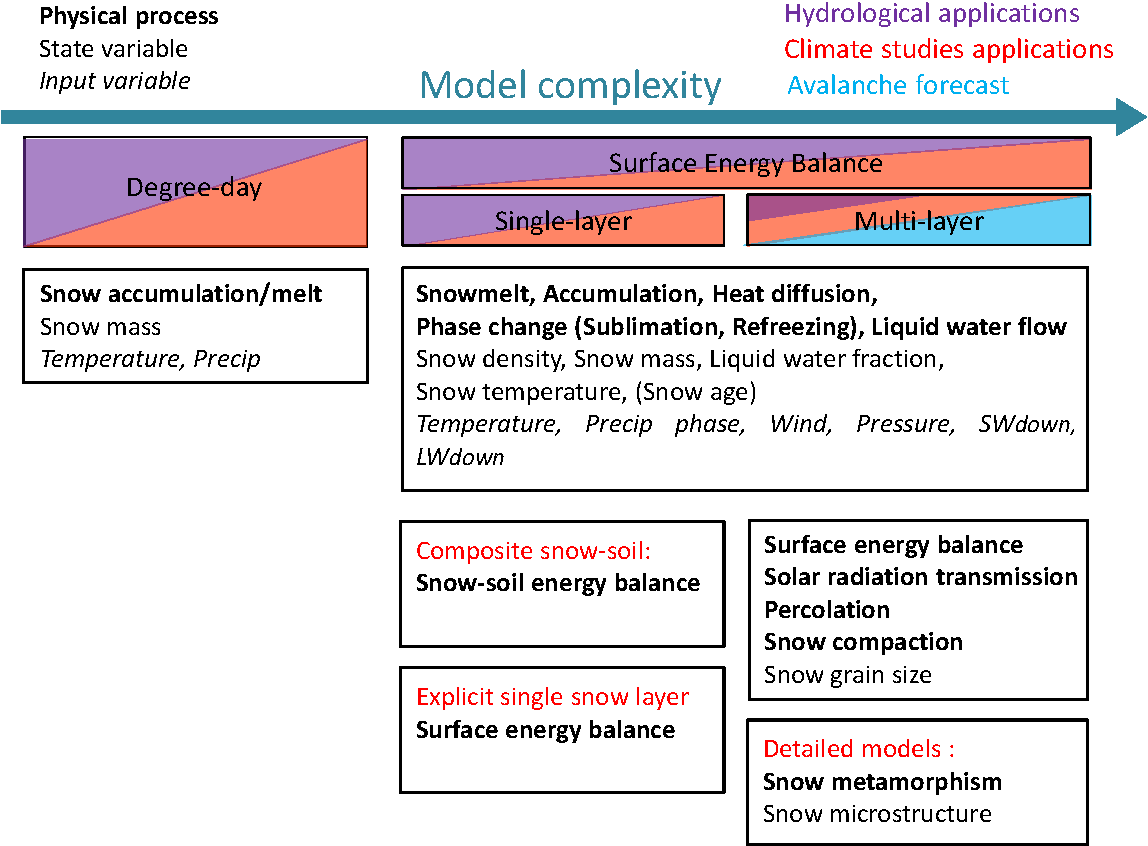
\includegraphics[scale=0.65]{Figures/Fig_modelcomplexity_AB}
	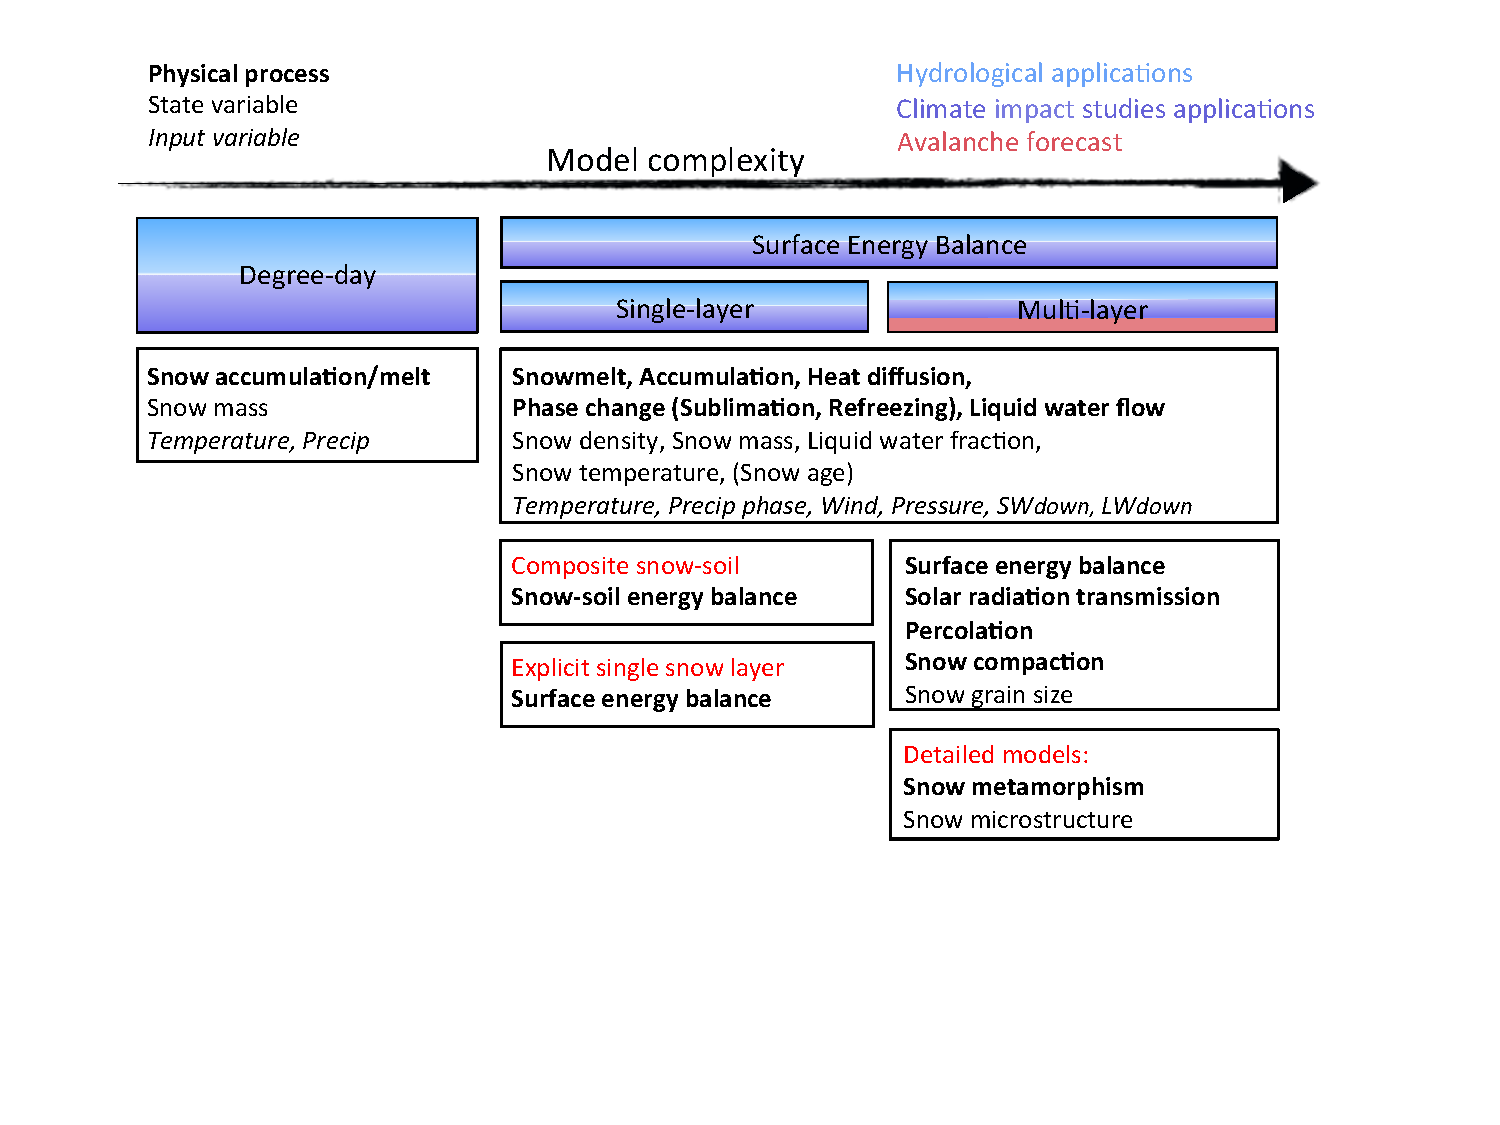
\includegraphics[scale=0.65]{Figures/Fig_modelcomplexity-Article-final}
	\caption{Description of snow physical processes (bold), state variables (regular) and input variables (italic) required per category of snow models complexity}\label{Fig:Model_complexity}
\end{figure}


\section{Uncertainties and limits associated to snow models} 

The representation of snow physical processes in snow models are associated to uncertainties related to the physical representation of the snow, where the precision is usually related to the complexity of the model but also from the meteorological data used. The uncertainties of a model are also related to the sub-grid variability of the study area, especially in complex mountainous terrain, such as topography and slope and non-represented processes such as lateral redistribution of snow by wind.
 

\subsection{Meteorological errors}

Snow models require meteorological forcings data as input, and model results depend significantly on the quality of the driving file.
Meteorological forcing data from NWP model output contains errors impacting snow model behaviour. This can be reduced through data assimilation in atmospheric reanalyses such as ERA-Interim \citep{Dee_2011}, or at a more local scale, SAFRAN \citep{Durand_1993}. Meteorological input plays a major role for the error budget of the modelling tools, which are often the dominating source of uncertainties of snow models \citep{Fekete_2004,Bosilovich_2008,Raleigh_2015,Essery_2013,Magnusson_2015}.



\subsection{Model errors}


\subsubsection{Ensemble simulations}

Model errors are due to a variety of reasons, including, in addition to meteorological forcing errors, the uncertainties pertaining to the initial conditions and parameterisations leading to a model errors. Multi-physics modelling systems use different combination of physical options. %To quantify the various contributions to the overall error distribution of the model, ensemble simulation made a large number of runs where each member uses slightly different initial conditions or physical options.
Ensemble simulations can be used to quantify the snow models errors due to the various contributions to the overall error distribution of the model. The latter is estimated through a large number of runs where each member uses slightly different initial conditions or physical options.
Multiple physics ensemble system, such as ESCROC \citep{Lafaysse_2017}, can be combined with ensemble NWP such as PEARP or PEAROME to represent both uncertainties in the snow model and in the meteorological forcings \citep{vernay2015}.


\subsubsection{Model-intercomparisons}

Model-intercomparison aims to better understand the difference between snow models that feature a wide complexity range. Physical snow processes in snow models are represented through different equations and parameterisations. Model-intercomparison projects such as ESM-SnowMIP (Snow Models Intercomparison Projects ) \citep{Krinner_2018} include a large variety of models which are diversely suited to various climate conditions. The prediction of snow accumulation and ablation differs from snow models, which leads to more significant difference during the snowmelt period \citep{Etchevers_2004}. This enhances a lower performance of the model during warmer winter and warmer sites due to higher frequency of melt-events \citep{Etchevers_2004}.


The different parameterisations leads to a spread of the evolution of the snowpack. 
The study of the spread between various model configurations illustrates that there is not only one configuration which provides the best simulations but an ensemble of configuration that yield good results and some configurations systematically providing inadequate results \citep{Essery_2013}. Models including prognostic snow density and albedo were shown to lead to better performance \citep{Essery_2013,Boone_2004}. The best simulations in terms of snow mass use an hydrological option which retain melt water. Additionally, snow depth is underestimated when configurations melt too early and is overestimated when snow density is underestimated \citep{Essery_2013}. Model performance is much more consistent at open sites than forest-sites \citep{Rutter_2009}. In the most recent model intercomparison ESM-SnowMIP project \citep{Krinner_2018}, the results shows, for all sites and all years, that the most detailed multi-layer snow models, such as Crocus, was one of the best performing models. 

Comparative studies have been carried out with different versions of snow models of Météo-France \citep{Boone_2001,Vionnet_2012,Decharme_2016}. The inclusion of the physical processes such as retention of liquid water in the multilayer model ISBA-ES resulted in an increase of the snowmelt runoff, which lead to better simulate SWE compared to the single snow layer of ISBA \citep{Boone_2001}. Due to a larger holding water capacity and condensation, Crocus simulates the largest SWE of the three models coupled to SURFEX, especially in high-latitudes. The integration of Crocus into ISBA (ISBA-Crocus), which represents snow-vegetation interaction, has lead to a better estimation of SWE \citep{Vionnet_2012}. 



%\subsection{Conclusion}
%Snow models can feature a wide complexity range, where the physical snow processes are represented through different equations and parameterisations. Model-intercomparison projects such as ESM-SnowMIP \citep{Krinner_2018} include a large variety of models which are diversely suited to various climate conditions. 
%Ensemble approaches are increasingly common to estimate uncertainties pertaining to model output, helping to better describe the best configurations options and the mechanisms behind model performance. When a model configuration is adjusted using observations, the performance of the model generally increases and leads to reduce the error and bias of the model \citep{Essery_2013}. 

%%%%%%%%%%%%%%%%%%%
%%%%% THE END %%%%%

%% optional
%\supplementary{The following are available online at \linksupplementary{s1}, Figure S1: title, Table S1: title, Video S1: title.}

% Only for the journal Methods and Protocols:
% If you wish to submit a video article, please do so with any other supplementary material.
% \supplementary{The following are available at \linksupplementary{s1}, Figure S1: title, Table S1: title, Video S1: title. A supporting video article is available at doi: link.}

%%%%%%%%%%%%%%%%%%%%%%%%%%%%%%%%%%%%%%%%%%
\authorcontributions{For research articles with several authors, a short paragraph specifying their individual contributions must be provided. The following statements should be used ``conceptualization, X.X. and Y.Y.; methodology, X.X.; software, X.X.; validation, X.X., Y.Y. and Z.Z.; formal analysis, X.X.; investigation, X.X.; resources, X.X.; data curation, X.X.; writing--original draft preparation, X.X.; writing--review and editing, X.X.; visualization, X.X.; supervision, X.X.; project administration, X.X.; funding acquisition, Y.Y.'', please turn to the  \href{http://img.mdpi.org/data/contributor-role-instruction.pdf}{CRediT taxonomy} for the term explanation. Authorship must be limited to those who have contributed substantially to the work reported.}

%%%%%%%%%%%%%%%%%%%%%%%%%%%%%%%%%%%%%%%%%%
\funding{This research was funded by NAME OF FUNDER grant number XXX.'' and ``The APC was funded by XXX''. Check carefully that the details given are accurate and use the standard spelling of funding agency names at \url{https://search.crossref.org/funding}, any errors may affect your future funding.}

%%%%%%%%%%%%%%%%%%%%%%%%%%%%%%%%%%%%%%%%%%
\acknowledgments{In this section you can acknowledge any support given which is not covered by the author contribution or funding sections. This may include administrative and technical support, or donations in kind (e.g., materials used for experiments).}

%%%%%%%%%%%%%%%%%%%%%%%%%%%%%%%%%%%%%%%%%%
\conflictsofinterest{The authors declare no conflict of interest.} 

%%%%%%%%%%%%%%%%%%%%%%%%%%%%%%%%%%%%%%%%%%
%% optional
%\abbreviations{The following abbreviations are used in this manuscript:\\
%
%\noindent 
%\begin{tabular}{@{}ll}
%DA & Data Assimilation\\
%SWE & Snow Water Equivalent\\
%\end{tabular}}

%%%%%%%%%%%%%%%%%%%%%%%%%%%%%%%%%%%%%%%%%%
%% optional
%\appendixtitles{no} %Leave argument "no" if all appendix headings stay EMPTY (then no dot is printed after "Appendix A"). If the appendix sections contain a heading then change the argument to "yes".
%\appendix
%\section{}
%\unskip
%\subsection{}



%%%%%%%%%%%%%%%%%%%%%%%%%%%%%%%%%%%%%%%%%%
% Citations and References in Supplementary files are permitted provided that they also appear in the reference list here. 

%=====================================
% References, variant A: internal bibliography
%=====================================
\reftitle{References}


%\begin{thebibliography}{999}
%% Reference 1
%\bibitem[Author1(year)]{ref-journal}
%Author1, T. The title of the cited article. {\em Journal Abbreviation} {\bf 2008}, {\em 10}, 142--149.
%% Reference 2
%\bibitem[Author2(year)]{ref-book}
%Author2, L. The title of the cited contribution. In {\em The Book Title}; Editor1, F., Editor2, A., Eds.; Publishing House: City, Country, 2007; pp. 32--58.
%\end{thebibliography}

% The following MDPI journals use author-date citation: Arts, Econometrics, Economies, Genealogy, Humanities, IJFS, JRFM, Laws, Religions, Risks, Social Sciences. For those journals, please follow the formatting guidelines on http://www.mdpi.com/authors/references
% To cite two works by the same author: \citeauthor{ref-journal-1a} (\citeyear{ref-journal-1a}, \citeyear{ref-journal-1b}). This produces: Whittaker (1967, 1975)
% To cite two works by the same author with specific pages: \citeauthor{ref-journal-3a} (\citeyear{ref-journal-3a}, p. 328; \citeyear{ref-journal-3b}, p.475). This produces: Wong (1999, p. 328; 2000, p. 475)

%=====================================
% References, variant B: external bibliography
%=====================================
\externalbibliography{yes}
\bibliography{BiblioSWE}
%%%%%%%%%%%%%%%%%%%%%%%%%%%%%%%%%%%%%%%%%%
%% optional
%\sampleavailability{Samples of the compounds ...... are available from the authors.}

%% for journal Sci
%\reviewreports{\\
%Reviewer 1 comments and authors’ response\\
%Reviewer 2 comments and authors’ response
%}

%%%%%%%%%%%%%%%%%%%%%%%%%%%%%%%%%%%%%%%%%%
\end{document}

